\documentclass[a4paper,11pt,openright]{report}
\setlength{\parindent}{0pt} % set noindent for entire file

\usepackage[utf8]{inputenc}
\usepackage[a4paper, left=10mm, right=10mm, top=20mm]{geometry}
\usepackage{xcolor,graphicx}
\usepackage{amsmath}
\usepackage{setspace}
\usepackage{sectsty}
\usepackage{etoolbox}
\usepackage{enumitem}
\usepackage{listings}
\usepackage{times}

\graphicspath{ {/home/saran/Analytics/May_01/} }

\lstdefinestyle{mystyle}{
	backgroundcolor=\color{white},
	basicstyle=\ttfamily\footnotesize,
	breakatwhitespace=false,
	breaklines=true,
	captionpos=b,
	keepspaces=true,
	showspaces=false,
	showstringspaces=false,
	showtabs=false,
	tabsize=4
}

\lstset{style=mystyle}

\begin{document}
\singlespacing
\pagestyle{plain}

\begin{center}
\textbf{Answers to Question Set 10} \\
Date: 01/05/2020 \hspace{2mm} Name: D.Saravanan
\end{center}

\vspace{10px}

\begin{enumerate}

\item[1.] Write a python program to get input from the user. \\

Program:
\lstinputlisting[language=Python]{question1.py}

\vspace{5px}

Output:
\lstinputlisting{output1.txt}

\vspace{10px}

\pagebreak

\item[2.] Display the growth percentage for the number of countries given by the user
sorted based on the mean GDP per capita. \\

Program:
\lstinputlisting[language=Python]{question2.py}

\vspace{5px}

\pagebreak

Output:
\lstinputlisting{output2.txt}

\vspace{10px}

\pagebreak

\item[3.] Plot a bar plot of the growth percentage. \\

Program: 
\lstinputlisting[language=Python]{question3.py}

\vspace{5px}

\pagebreak

Output:
%figure_1
\begin{figure}[ht!]
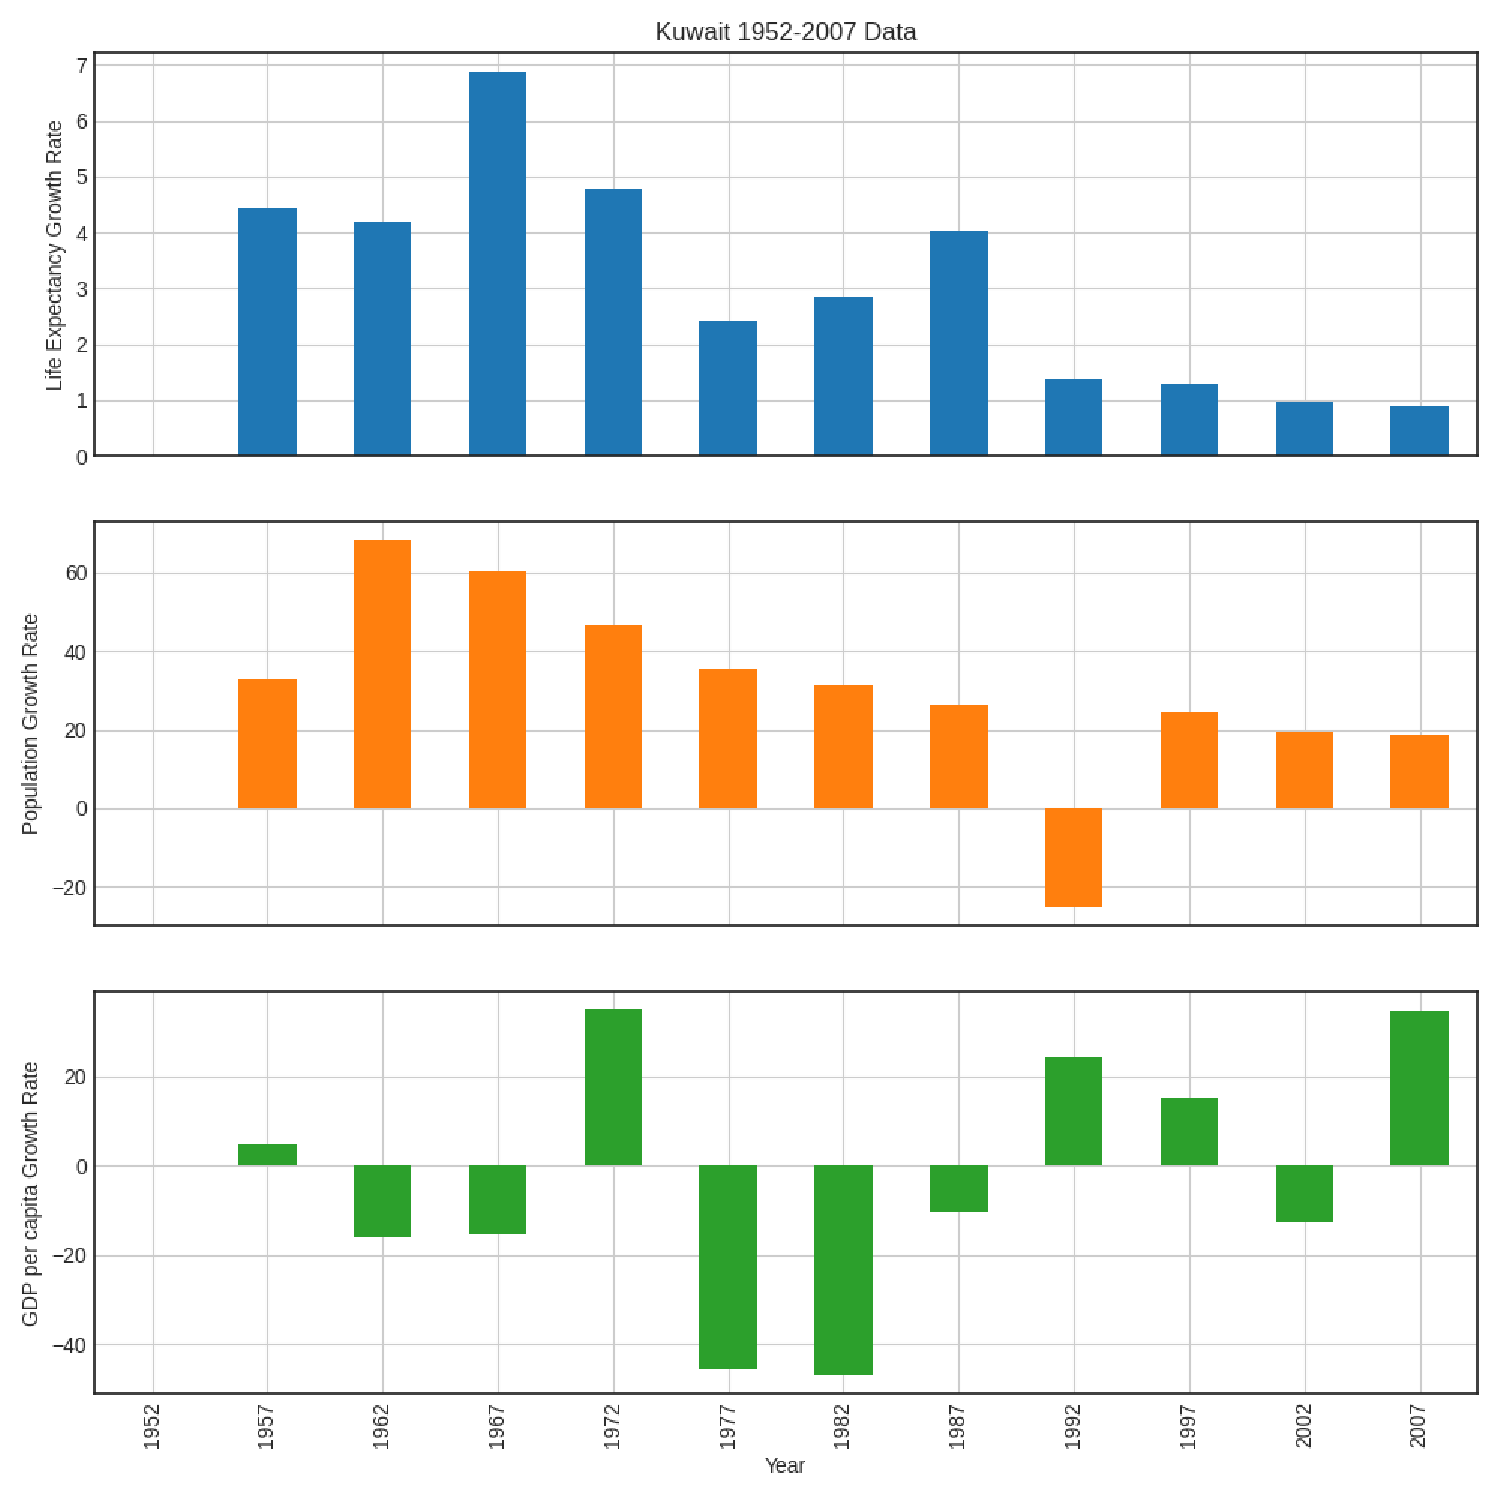
\includegraphics[width=30cm,height=15cm,keepaspectratio]{Kuwait.pdf}
\centering
\end{figure}

%figure_2
\begin{figure}[ht!]
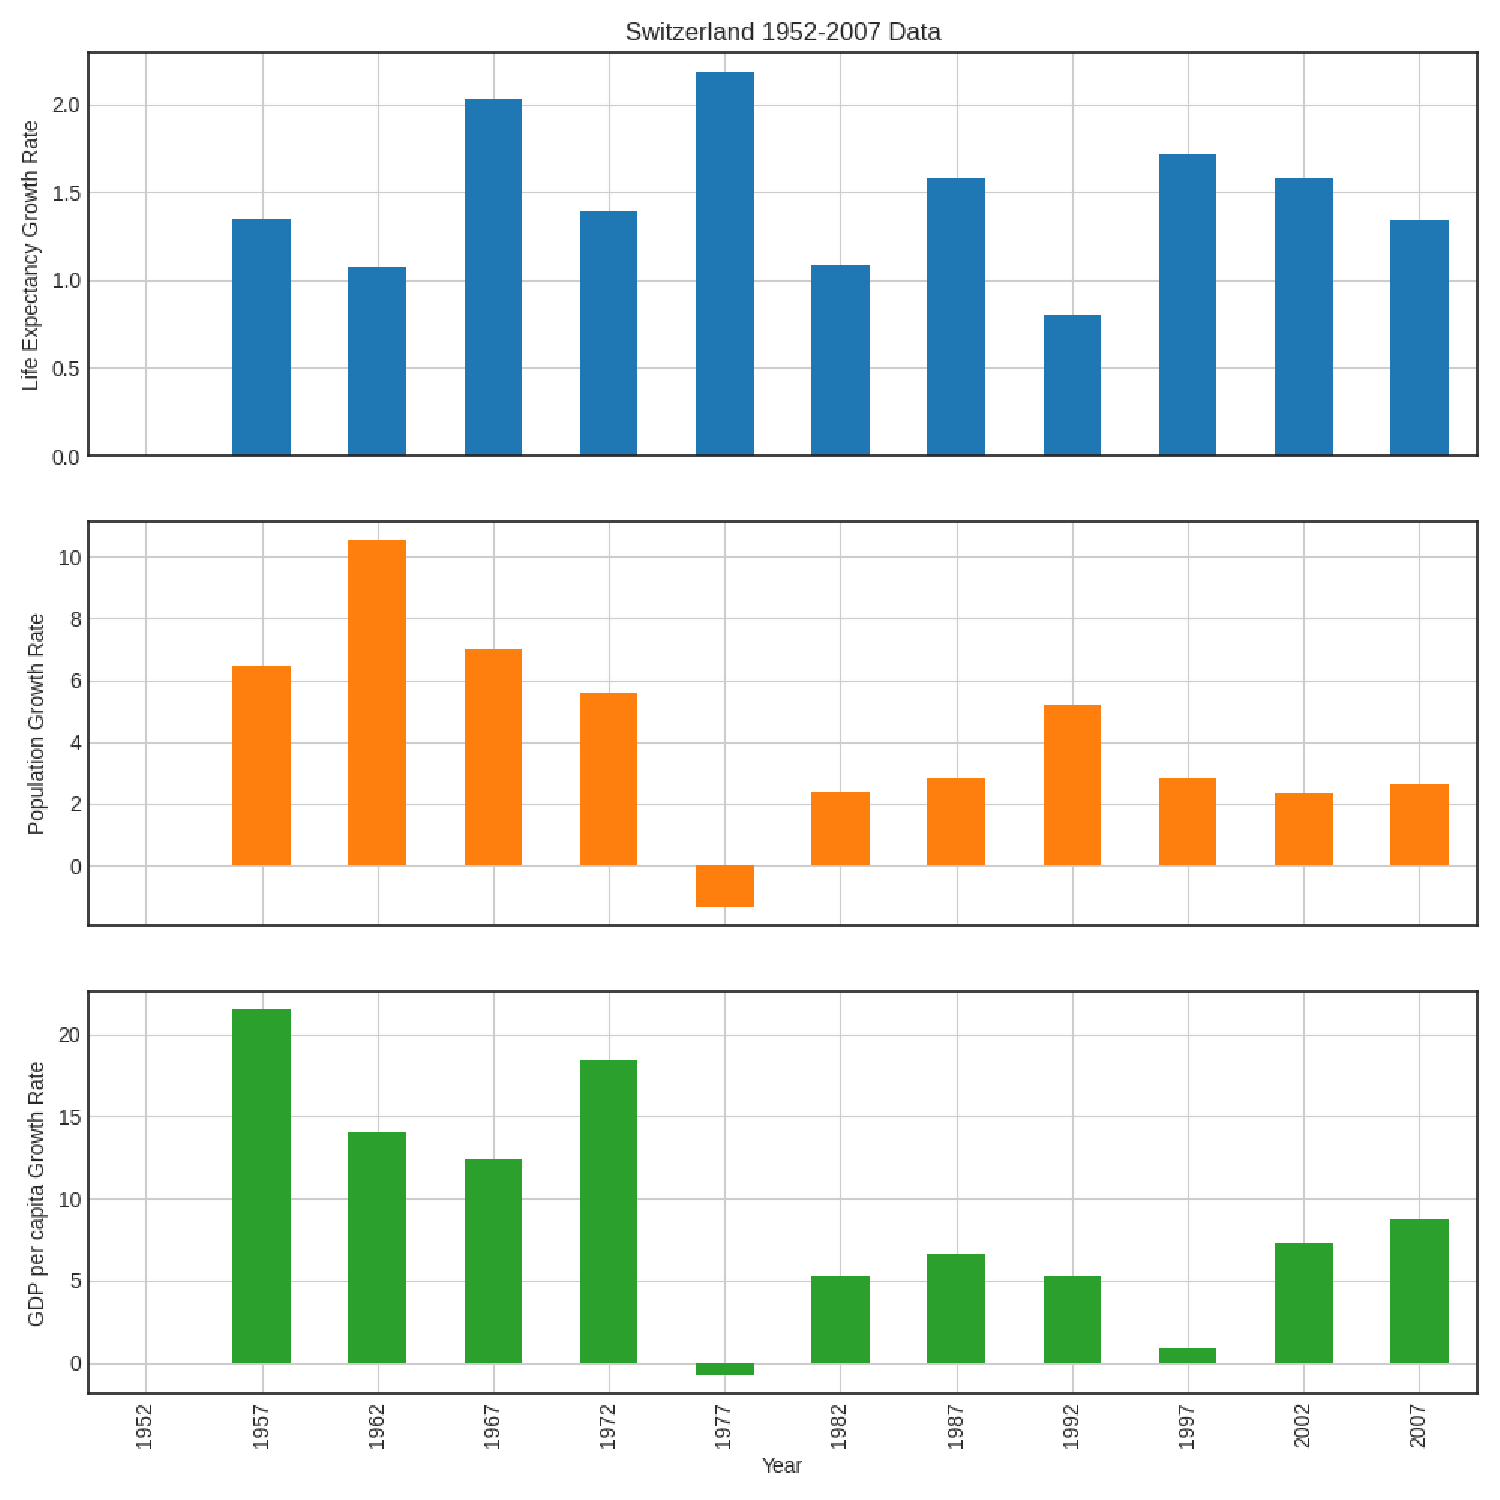
\includegraphics[width=30cm,height=15cm,keepaspectratio]{Switzerland.pdf}
\centering
\end{figure}

%figure_3
\begin{figure}[ht!]
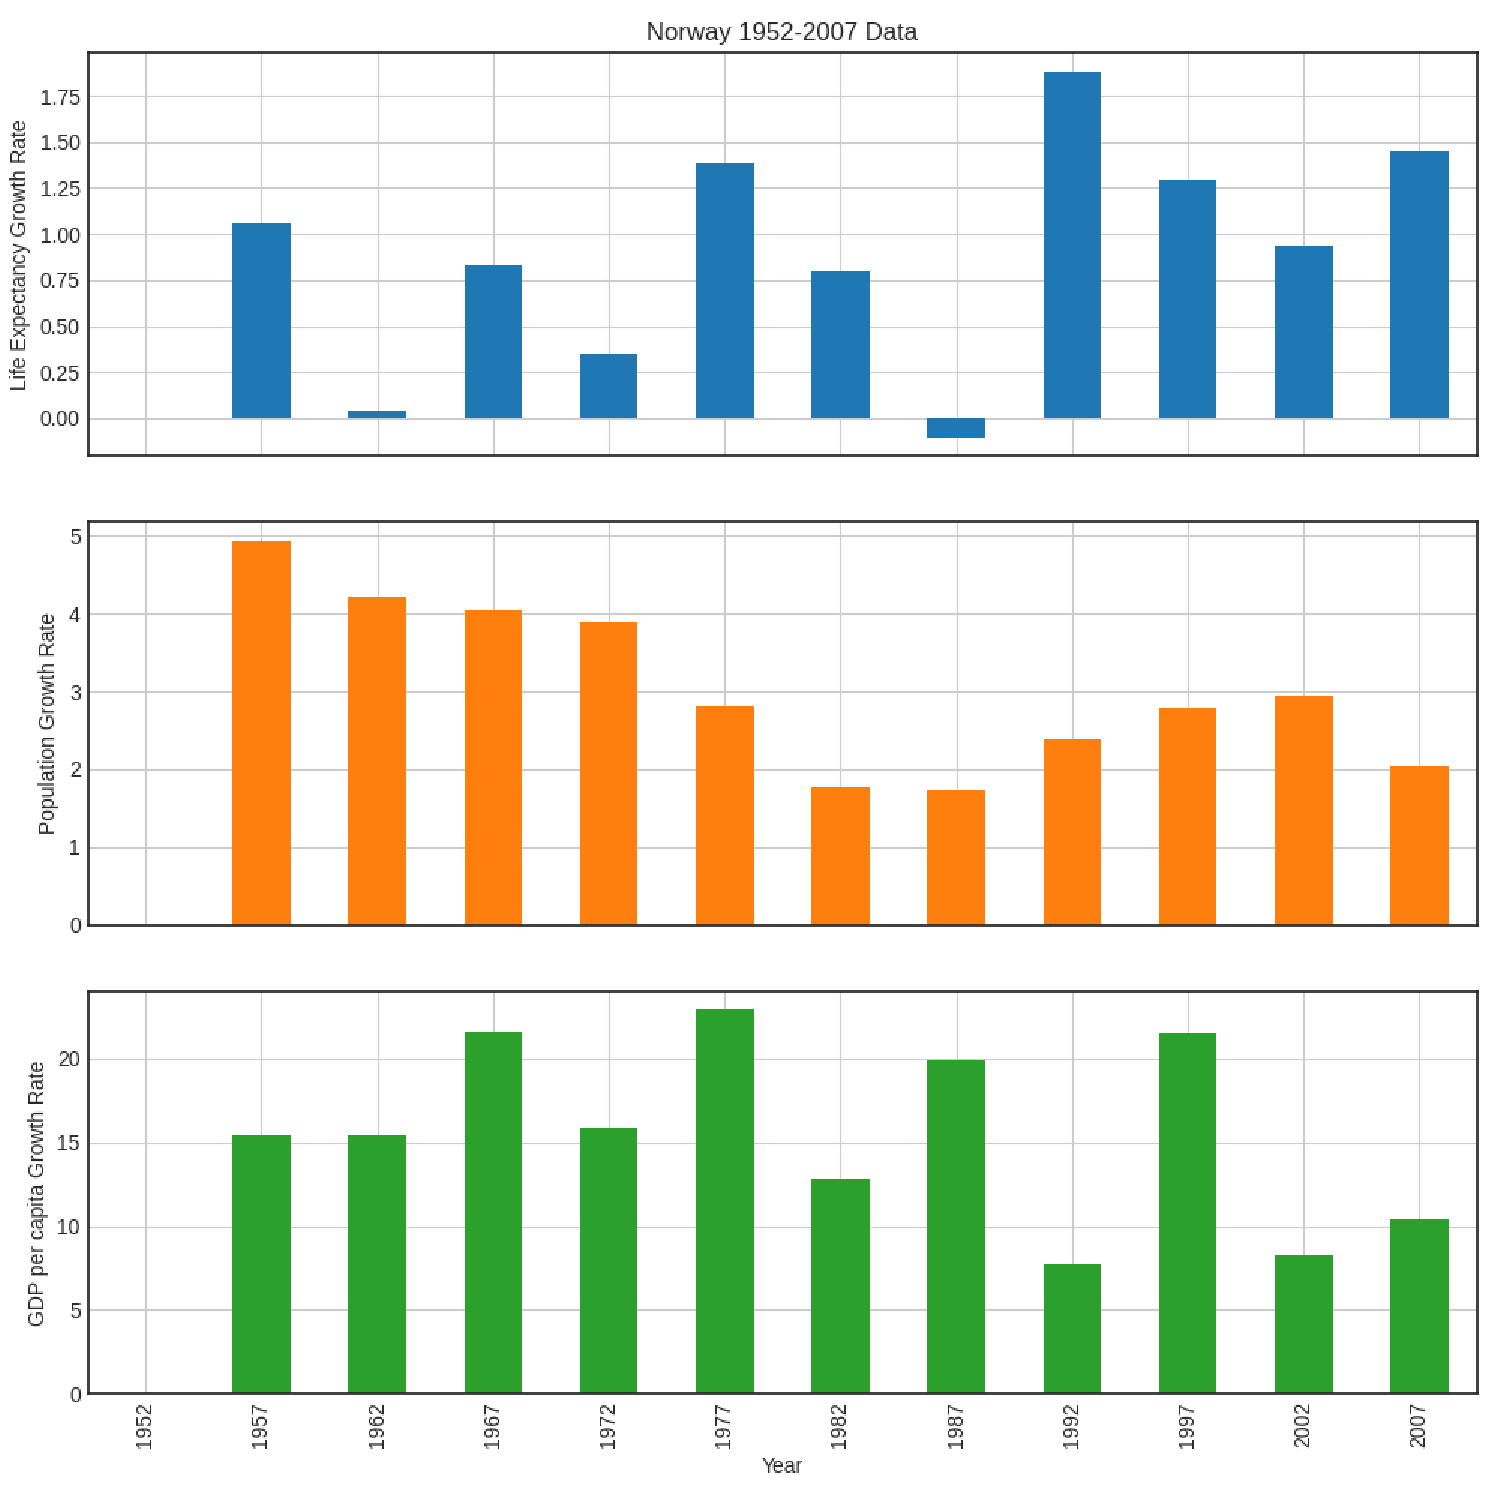
\includegraphics[width=30cm,height=15cm,keepaspectratio]{Norway.pdf}
\centering
\end{figure}

\end{enumerate}

\end{document}
